\newpage
\def\thoigian{90}%--Thời gian
\de{Đề số 2}{Chương VI. Hàm số mũ và hàm số lôgarit}


\ind{PHẦN I.} \inden{Câu trắc nghiệm nhiều phương án lựa chọn. Mỗi câu hỏi học sinh chỉ chọn một phương án.}\\
\setcounter{ex}{0}
\Opensolutionfile{ans}[ans/1D6-OTC-D2-1]
\setcounter{ex}{0}
\begin{ex}%[1D6N1-4]
	Cho hai số thực $\alpha$, $\beta$ thỏa mãn $\left(0{,}25\pi\right)^{\alpha}>\left(0{,}25\pi\right)^{\beta}$. Khẳng định nào sau đây đúng?
	\choice
	{$\alpha\cdot \beta=1$}
	{$\alpha>\beta$}
	{$\alpha+\beta=0$}
	{\True $\alpha<\beta$}
	\loigiai{
		Do $0<0{,}25\pi<1$ nên $\left(0{,}25\pi\right)^{\alpha}>\left(0{,}25\pi\right)^{\beta}\Leftrightarrow \alpha <\beta$.
	}
\end{ex}
\begin{ex}%[1D6N1-2]
	Tính giá trị biểu thức $A = \dfrac{6^{3+\sqrt{5}}}{2^{2+\sqrt{5}}\cdot 3^{1+\sqrt{5}}}$.
	\choice
	{$1$}
	{$6^{-\sqrt{5}}$}
	{\True $18$}
	{$9$}
	\loigiai{
		Ta có $A = \dfrac{6^{3+\sqrt{5}}}{2^{2+\sqrt{5}}\cdot 3^{1+\sqrt{5}}}=\dfrac{2^{3+\sqrt{5}}\cdot 3^{3+\sqrt{5}}}{2^{2+\sqrt{5}}\cdot 3^{1+\sqrt{5}}}=2\cdot 3^2 =18$.
	}
\end{ex}
\begin{ex}%[1D6N1-2]
	Biến đổi $\sqrt[3]{x^5.\sqrt[4]{x}}$, $(x>0)$ thành dạng lũy thừa với số mũ hữu tỉ ta được
	\choice
	{${x}^{\tfrac{20}{3}}$}
	{${x}^{\tfrac{23}{12}}$}
	{\True ${x}^{\tfrac{21}{12}}$}
	{${x}^{\tfrac{12}{5}}$}
	\loigiai{Với $x>0$ ta có $\sqrt[3]{x^5.\sqrt[4]{x}}=\sqrt[3]{x^5\cdot x^{\tfrac{1}{4}}}=\sqrt[3]{x^{5+\tfrac{1}{4}}}=\left(x^{\tfrac{21}{4}}\right)^{\tfrac{1}{3}}=x^{\tfrac{21}{4}\cdot\tfrac{1}{3}}=x^{\tfrac{21}{12}}$.
	}
\end{ex}
\begin{ex}%[1D6N2-2]
	Cho $a$, $b>0$. Tìm mệnh dề đúng trong các mệnh đề sau.
	\choice
	{\True $\ln \dfrac{a}{b}=\ln a+\ln \dfrac{1}{b}$}
	{$\ln \dfrac{a}{b}=\ln b-\ln a$}
	{$\ln \dfrac{a}{b}=\dfrac{\ln a}{\ln b}$}
	{$\ln \dfrac{a}{b}=\ln a-\ln \dfrac{1}{b}$}
	\loigiai{
		Ta có $\ln \dfrac{a}{b}=\ln \left(a\cdot \dfrac{1}{b}\right)=\ln a+\ln \dfrac{1}{b}.$
	}
\end{ex} 

\begin{ex}%[1D6N2-1]
	Giá trị của biểu thức $A=4^{\log_27}$ bằng
	\choice
	{$14$}
	{$28$}
	{$2$}
	{\True $49$}
	\loigiai{ Ta có $A=4^{\log_27}=2^{2\log_27}=2^{\log_27^2}=49$.
	}
\end{ex}
\begin{ex}%[1D6N2-2]
	Cho $a>0$, $a\neq 1$ giá trị của biểu thức $\log_{\frac{1}{a}}\sqrt[3]{a^7}$ là
	\choice
	{$-\dfrac{3}{7}$}
	{$\dfrac{7}{3}$}
	{$\dfrac{3}{7}$}
	{\True $-\dfrac{7}{3}$}
	\loigiai{
		Có $\log_{\frac{1}{a}}\sqrt[3]{a^7}=\log_{a^{-1}}a^{\frac{7}{3}}=-\dfrac{7}{3}$.
	} 
\end{ex}
\begin{ex}%[1D6N3-2]
	Tập xác định của hàm số $y=9^x$ là
	\choice
	{\True $\mathbb R$}
	{$[0;+\infty)$}
	{$\mathbb R\setminus\{0\}$}
	{$(0;+\infty)$}
	\loigiai{
	Với $a>0$ và $a \ne 1$
		\begin{itemize}
			\item [$\bullet$] Hàm số $y=a^x$ có tập xác định là $\mathbb{R}$.
			\item [$\bullet$]  Hàm số $y=a^x$ có tập giá trị là $(0;+\infty)$.
		\end{itemize}
	}
\end{ex}
\begin{ex}%[1D6N3-2]
	Tập xác định của hàm số $y=\log_3{x}$ là
	\choice
	{$\left[0;+\infty \right)$}
	{$\mathbb{R}\setminus {\left\lbrace 0\right\rbrace}$}
	{$\mathbb{R}$}
	{\True $\left(0;+\infty \right)$}
	\loigiai{
		Hàm số $y=\log_3{x}$ xác định trên $\left(0;+\infty \right)$.
	}
\end{ex}
\begin{ex}%[1D6H3-4]
	\immini[thm]{Cho $a$, $b$, $c$ là các số thực dương, khác 1. Đồ thị các hàm số $y=a^x$, $y=b^x$, $y=c^x$ được cho trong hình vẽ bên. Mệnh đề nào sau đây đúng?
		\choice
		{$1<a<c<b$}
		{\True $a<1<c<b$}
		{$a<1<b<c$}
		{$1<a<b<c$}}
	{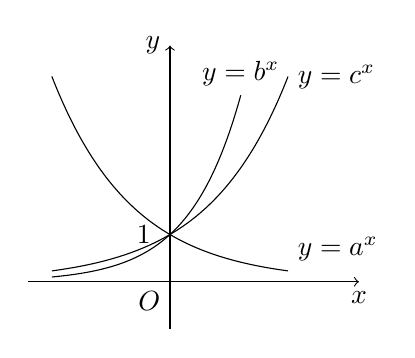
\begin{tikzpicture}[scale=0.6]
			\draw[->] (-3,0)--(0,0) node[below left]{$O$}--(4,0) node[below] {$x$};
			\draw[->] (0,-1)-- (0,5) node[left]{$y$};
			\node[left] at (-.2,1) {$1$};
			\draw[smooth,samples=100,domain=-2.5:2.5] plot(\x,{1/(1.8^(\x))}) node[above right]{$y=a^x$};
			\draw[smooth,samples=100,domain=-2.5:1.5] plot(\x,{2.5^(\x)}) node[above]{$y=b^x$};
			\draw[smooth,samples=100,domain=-2.5:2.5] plot(\x,{1.8^(\x)}) node[right]{$y=c^x$};
	\end{tikzpicture}}
	\loigiai{\immini{Xét đường thẳng $x=1$. Nó cắt các đường cong $y=a^x$, $y=b^x$, $y=c^x$, $y=1$ lần lượt tại các điểm mà tung độ là $a$, $b$, $c$, $1$. Căn cứ vào đồ thị đã cho, ta suy ra $a<1<c<b.$}
		{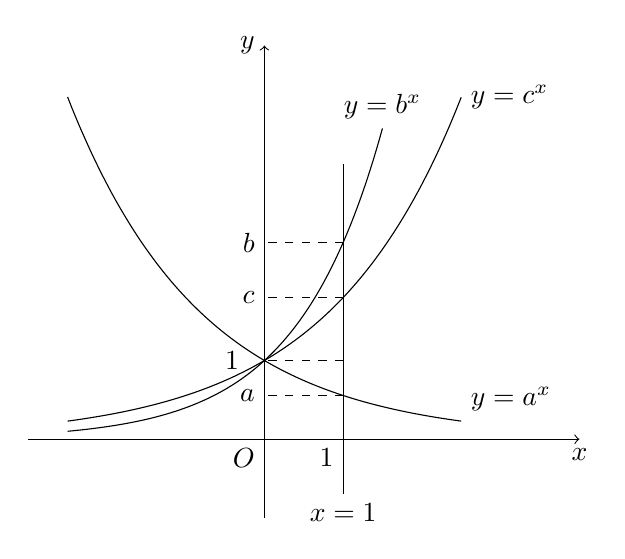
\begin{tikzpicture}
				\draw[->] (-3,0)--(0,0) node[below left]{$O$}--(4,0) node[below] {$x$};
				\draw[->] (0,-1)-- (0,5) node[left]{$y$};
				\node[left] at (-.2,1) {$1$};
				\draw[-](1,-.7) node[below]{$x=1$}--(1,0) node[below left]{$1$}--(1,3.5);
				\draw[-][dashed](1,.5556)--(0,.5556) node[left]{$a$};
				\draw[-][dashed](1,1.8)--(0,1.8) node[left]{$c$};
				\draw[-][dashed](1,2.5)--(0,2.5) node[left]{$b$};
				\draw[-][dashed](1,1)--(0,1);
				\draw[smooth,samples=100,domain=-2.5:2.5] plot(\x,{1/(1.8^(\x))}) node[above right]{$y=a^x$};
				\draw[smooth,samples=100,domain=-2.5:1.5] plot(\x,{2.5^(\x)}) node[above]{$y=b^x$};
				\draw[smooth,samples=100,domain=-2.5:2.5] plot(\x,{1.8^(\x)}) node[right]{$y=c^x$};
			\end{tikzpicture}
		}
	}
\end{ex}
\begin{ex}%[1D6N4-2]
	Phương trình $2^{2x+1}=32$ có nghiệm là
	\choice
	{$x=\dfrac{5}{2}$}
	{\True $x=2$}
	{$x=\dfrac{3}{2}$}
	{$x=3$}
	\loigiai{
		Ta có $2^{2x+1}=32 \Leftrightarrow 2x+1=5 \Leftrightarrow x=2$.}
\end{ex}
\begin{ex}%[1D6H4-2]
	Tập nghiệm của phương trình $\log_2(x^2-1)=3$ là
	\choice
	{\True $\{-3;3\}$}
	{$\{-3\}$}
	{$\{3\}$}
	{$\left\lbrace -\sqrt{10};\sqrt{10}\right\rbrace $}
	\loigiai{
		Ta có $\log_2(x^2-1)=3 \Leftrightarrow x^2-1=2^3\Leftrightarrow \hoac{&x=3\\&x=-3.}$\\
		Vậy tập nghiệm của phương trình đã cho là $ \lbrace -3; 3\rbrace $.
	}
\end{ex}
\begin{ex}%[1D6N4-3]
	Giải  bất  phương trình $\log_2(3x-2)>\log_2(6-5x)$ được tập nghiệm là $(a;b)$. Giá trị của biểu thức $a+b$.
	\choice
	{$S=\dfrac{26}{5}$}
	{$S=\dfrac{8}{3}$}
	{$S=\dfrac{28}{15}$}
	{\True $S=\dfrac{11}{5}$}
	\loigiai{
	Ta có	$\log_2(3x-2)>\log_2(6-5x)\Leftrightarrow \heva{&3x-2>0\\&6-5x>0\\&3x-2>6-5x}\Leftrightarrow \heva{&x>\dfrac{2}{3}\\&x<\dfrac{6}{5}\\&x>1}\Leftrightarrow 1<x<\dfrac{6}{5}$. 
	\\Do đó tập nghiệm của bất phương trình là $S=\left(1;\dfrac{6}{5}\right)$. 
	\\Vậy $a+b=1+\dfrac{6}{5}=\dfrac{11}{5}.$	
	}
\end{ex}

\Closesolutionfile{ans}

\ind{PHẦN II.} \inden{Câu trắc nghiệm đúng sai. Trong mỗi ý a), b), c), d) ở mỗi câu, học sinh chọn đúng hoặc sai.}\\
\Opensolutionfile{ans}[ans/1D6-OTC-D2-2]
\setcounter{ex}{0}
\begin{ex}%[1D6H3-3]
	Cho các hàm số $y=\log_{{}a}x$, $y=a^x$ với $a$ là số thực dương khác $1$.
	\choiceTF
	{\True Đồ thị hàm số $y=\log_{{}a}x$ nằm bên phải trục tung}
	{Hàm số $y=\log_{{}a}x$ và hàm số $y=a^x$ có cùng tập giá trị}
	{\True Hàm số $y=a^x$ với $0<a<1$ nghịch biến trên khoảng $(-\infty;+\infty)$}
	{Đồ thị hàm số $y=a^x$ với $a>0$ và $a\ne 1$ luôn đi qua điểm $A(a;1)$}
	\loigiai{\begin{itemchoice}
			\itemch Do $x>0$ nên đồ thị hàm số $y=\log_{{}a}x$ nằm bên phải trục tung.
			\itemch Hàm số $y=a^x$ có tập giá trị là $(0;+\infty)$ còn hàm số $y=\log_{{}a}x$ có tập giá trị là $(-\infty;+\infty)$.
			\itemch Hàm số $y=a^x$ với $0<a<1$ nghịch biến trên khoảng $(-\infty;+\infty)$.
			\itemch Đồ thị hàm số $y=a^x$ với $a>0$ và $a\ne 1$ luôn đi qua điểm $A(0;1)$.
		\end{itemchoice}
	} 
\end{ex}
\begin{ex}%[1D6V4-4]
	Cho hàm số $f(x)=\left(\dfrac{1}{3} \right)^x$.
	\choiceTF
	{\True $f(-2)=9$}
	{Tập xác định của hàm số $f(x)$ là $\mathscr{D}=(0;+\infty)$}
	{\True Phương trình $f(x)=m$ có nghiệm khi và chỉ khi $\,m > 0$}
	{Tập nghiệm của bất phương trình $f(x) > 27^{x^2}$ là $S=\left(-1;-\dfrac{1}{3} \right)$}
	\loigiai{
		\begin{itemchoice}
			\itemch Ta có $f(-2)=\left(\dfrac{1}{3} \right)^{-2}=3^2=9$.
			\itemch Tập xác định $\mathscr{D}=\mathbb{R}$.
			\itemch  
			Xét phương trình $\left(\dfrac{1}{3} \right)^x=m$.\\
			Vì $\left(\dfrac{1}{3} \right)^x>0$, $\forall x \in \mathbb{R}$ nên phương trình có nghiệm khi và chỉ khi  $m>0$.
			\itemch 
			Ta có
			\allowdisplaybreaks
			\begin{eqnarray*}
				& &f(x) > 27^{x^2}\\
				&\Leftrightarrow& \left(\dfrac{1}{3} \right)^x> 27^{x^2}\\
				&\Leftrightarrow& 3^{-x}>\left(3^3\right)^{x^2}\\
				&\Leftrightarrow& -x>3x^2\\
				&\Leftrightarrow& 3x^2+x<0\\
				&\Leftrightarrow& -\dfrac{1}{3}<x<0.
			\end{eqnarray*}
			Vậy $S=\left(-\dfrac{1}{3};0\right)$.
		\end{itemchoice}
	}
\end{ex}

\Closesolutionfile{ans}

\ind{PHẦN III.} \inden{Câu trắc nghiệm trả lời ngắn.}\\
\Opensolutionfile{ans}[ans/1D6-OTC-D2-3]
\setcounter{ex}{0}
\begin{ex}%[1D6V3-2]
	Có bao nhiêu giá trị nguyên của tham số $m<10$ để hàm số $y=\dfrac{1}{\sqrt{\log_3\left(x^2 - 2x + 3m\right)}}$ có tập xác định $\mathbb{R}$?\par
	\shortans{9}
	\loigiai{
		Hàm số $y=\dfrac{1}{\sqrt{\log_3\left(x^2 - 2x + 3m\right)}}$ có tập xác định $\mathbb{R}$ khi và chỉ khi 
		$$x^2 - 2x + 3m>1, \forall x\in \mathbb{R}\Leftrightarrow x^2 - 2x + 3m - 1>0, \forall x\in \mathbb{R}\Leftrightarrow 1 - 3m + 1<0\Leftrightarrow m>\dfrac{2}{3}.$$
	Vì $m\in\mathbb Z$ và $m<10$ nên $m\in\{0;1;2;\ldots;9\}$. }
\end{ex}
\begin{ex}%[1D6V4-2]
	Tổng các nghiệm của phương trình $\log_2^2 x - 2\log_2 x - 3 = 0$ bằng
	\shortans{8{,}5}
	\loigiai{Điều kiện $x>0$. Ta có \begin{align*}
			\log _2^2 x - 2\log _2 x - 3 = 0 & \Leftrightarrow (\log _2 x + 1)(\log_2 x - 3) = 0\\
			& \Leftrightarrow \hoac{&\log_2 x = -1\\& \log _2 x = 3}\\
			& \Leftrightarrow \hoac{& x = \dfrac{1}{2}\\ & x = 8.}
		\end{align*}
		Suy ra, tổng các nghiệm của phương trình đã cho bằng $\dfrac{1}{2} + 8 = \dfrac{17}{2}=8{,}5$.
	}
\end{ex}
\begin{ex}%[1D6V4-2]
	Tính tổng các nghiệm của phương trình $ 3\cdot 4^{x+1}-35\cdot 6^x+2\cdot 9^{x+1}=0 $.	
	\shortans{-1}
	\loigiai{
		Phương trình $ \Leftrightarrow 18\left(\dfrac{3}{2}\right)^{2x}-35\left(\dfrac{3}{2}\right)^x+12=0\Leftrightarrow \hoac{&
			\left(\dfrac{3}{2}\right)^x=\dfrac{3}{2}\\&
			\left(\dfrac{3}{2}\right)^x=\dfrac{4}{9}}\Leftrightarrow \hoac{&
			x=1\\&
			x=-2.} $
		\\
		Vậy tổng các nghiệm là $ -1 $.
		
	}
	
	
\end{ex}
\begin{ex}%[1D6V4-3]
	Có bao nhiêu số nguyên $ x $ thỏa mãn $\left(x^2-99 x-100\right)\ln (x-1)<0 $?
	\shortans{97}
	\loigiai{
		Bất phương trình đã cho
		\begin{eqnarray*}
			&&\left(x^2-99x-100\right)\ln (x-1)<0\\
			&\Leftrightarrow &\hoac{&\heva{& x^2-99x-100<0\\ &\ln (x-1)>0}\\ &\heva{& x^2-99x-100>0\\ &\ln (x-1)<0}}\\
			&\Leftrightarrow &\hoac{&\heva{&-1<x<100\\ & x>2}\\ &\heva{&\hoac{& x<-1\\ & x>100}\\ & 1<x<2}}\\
			&\Leftrightarrow & 2<x<100.
		\end{eqnarray*}
		Vì $ x $ nguyên nên $ x\in\{3; 4; 5; \ldots; 97; 98; 99\}$.\\
		Vậy có $ 97 $ giá trị nguyên của $ x $ thỏa mãn.
	}
\end{ex}
\Closesolutionfile{ans}
\ind{PHẦN IV.} \inden{Bài tập tự luận.}\\
\Opensolutionfile{ans}[ans/1D6-OTC-D2-4]
\setcounter{ex}{0}
\begin{ex}%[1D6V1-2]
	Cho số thực $x$ thỏa mãn $4^x + 4^{-x} = 14$. Tính $M = \dfrac{2 + 2^x + 2^{-x}}{7 - 2^x - 2^{-x}}$.
	\loigiai{
		Ta có $4^x + 4^{-x} = 14 \Leftrightarrow \left(2^x + 2^{-x}\right)^2 - 2\cdot 2^x\cdot 2^{-x} = 14 \Leftrightarrow \left(2^x + 2^{-x}\right)^2 = 16 \Rightarrow 2^x + 2^{-x} = 4$.\\
		Vậy $M = \dfrac{2 + 2^x + 2^{-x}}{7 - 2^x - 2^{-x}} = \dfrac{2 + 4}{7 -4} = 2$.
	}
\end{ex}
\begin{ex}%[1D6H4-5]
	Giải bất phương trình $\log_{3}\left(13-x^2\right)>2$.
	\loigiai{
		\allowdisplaybreaks
		\begin{eqnarray*}
			\log_{3}\left(13-x^2\right)>2&\Leftrightarrow& \heva{&13-x^2>0\\&13-x^2>3^2}\\
			&\Leftrightarrow& \heva{&-\sqrt{13}<x<\sqrt{13}\\&-2<x<2}\\
			&\Leftrightarrow& -2<x<2.
		\end{eqnarray*}
		Vậy tập nghiệm của bất phương trình đã cho là $S=(-2;2)$.
	}
\end{ex}
\begin{ex}%[1D6V5-5]
	Sự tăng trưởng của một loại vi khuẩn tuân theo công thức $S=A\cdot\mathrm{e}^{r\cdot t}$, trong đó $A$ là số lượng vi khuẩn ban đầu, $r$ là tỉ lệ tăng trưởng $\left(r>0\right)$, $t$ là thời gian tăng trưởng. Biết số lượng vi khuẩn ban đầu là $50$ con và sau $5$ giờ có được $250$ con. Hỏi sau ít nhất bao nhiêu giờ thì số vi khuẩn có được là trên $2$ triệu con (lấy số giờ là số nguyên)?
	\loigiai{
		Theo giả thiết thì số lượng vi khuẩn ban đầu là $50$ con và sau $5$ giờ là $250$ con, suy ra \[250=50\cdot\mathrm{e}^{r\cdot 5}\Leftrightarrow r=\dfrac{1}{5}\ln5.\]
		Lúc đó $S=50\cdot \mathrm{e}^{\left(\tfrac{1}{5}\ln5\right)t}$.\\
		Số vi khuẩn có được là trên $2$ triệu con khi
		\begin{eqnarray*}
			&&50\cdot\mathrm{e}^{\left(\tfrac{1}{5}\ln5\right)\cdot t}>2\,000\,000\\
			&\Leftrightarrow&\mathrm{e}^{\left(\tfrac{1}{5}\ln5\right)\cdot t}>40\,000\\
			&\Leftrightarrow&t>\dfrac{5\ln40\,000}{\ln 5}\approx 32{,}92.
		\end{eqnarray*}
		Vậy sau ít nhất $33$ giờ thì số vi khuẩn có được là trên $2$ triệu con.}
\end{ex}


\Closesolutionfile{ans}


